\documentclass[12pt,a4paper]{article}

 
\usepackage[utf8]{inputenc}
\usepackage[T1]{fontenc}
\usepackage[french]{babel}
\usepackage{amsmath, amssymb}
\usepackage{geometry}
\usepackage{xcolor}
\usepackage{tikz}
\usepackage{graphicx}
\usepackage{hyperref}
\usepackage{setspace}
\usepackage{fancyhdr}
\usepackage{tikz}
\usepackage{eso-pic}
\usepackage{listings}
\usepackage{xcolor}

\lstset{
    language=Python,
    basicstyle=\ttfamily\footnotesize,
    keywordstyle=\color{blue},
    commentstyle=\color{gray},
    stringstyle=\color{red!60!black},
    numbers=left,
    numberstyle=\tiny,
    stepnumber=1,
    numbersep=8pt,
    frame=single,
    breaklines=true,
    showstringspaces=false,
    captionpos=b
}

\geometry{
  top=2cm,
  bottom=2cm,
  left=2.5cm,
  right=2.5cm
}
 
\definecolor{bleufonce}{RGB}{0, 51, 102}
\definecolor{bleumoyen}{RGB}{0, 90, 160}
\definecolor{grisclair}{RGB}{230, 235, 240}
\definecolor{grisneutre}{RGB}{100, 110, 120}
 
\hypersetup{
  colorlinks=false,
  hidelinks
}

% Encodage et langue
\usepackage[utf8]{inputenc}
\usepackage[T1]{fontenc}
\usepackage[french]{babel}

% Mathématiques
\usepackage{amsmath, amssymb, amsthm}

% Mise en page
\usepackage{geometry}
\geometry{margin=2.5cm}

% Images et figures
\usepackage{graphicx}
\usepackage{float}

% Liens cliquables, optionnel mais utile
\usepackage{hyperref}

% Théorèmes
\newtheorem{theoreme}{Théorème}

\newtheorem{theorem}{Théorème}[section]
\newtheorem{lemma}[theorem]{Lemme}
 
\theoremstyle{remark}
\newtheorem*{remark}{Remarque}

% Titre du rapport
\author{}
\date{}


\begin{document}
\pagestyle{empty}
 
\begin{tikzpicture}[remember picture, overlay]
  % Bande bleue en haut
  \fill[bleufonce] (current page.north west) rectangle ++(\paperwidth,-3.5cm);
  % Fine ligne décorative sous la bande
  \fill[bleumoyen] (current page.north west)++(0,-3.5cm) rectangle ++(\paperwidth,-0.12cm);
  % Bande grise en bas
  \fill[grisclair] (current page.south west) rectangle ++(\paperwidth, 2.8cm);
  % Fine ligne décorative au-dessus de la bande du bas
  \fill[bleumoyen] (current page.south west)++(0,2.8cm) rectangle ++(\paperwidth,0.12cm);
\end{tikzpicture}
 
\vspace*{0.6cm}
 
% ---- En-tête (dans la bande bleue) ----
\begin{center}
  {\color{white}\fontsize{11}{14}\selectfont
    Université Sorbonne Paris Nord \quad$|$\quad Institut Galilée \quad$|$\quad Sup Galilée}\\[0.3cm]
  {\color{white!80!bleufonce}\fontsize{10}{13}\selectfont
     ING2 MACS --- Sup Galilée}
\end{center}
 
\vspace{2.8cm}
 
% ---- Filet décoratif ----
\begin{center}
  \begin{tikzpicture}
    \draw[bleumoyen, line width=1.2pt] (0,0) -- (14,0);
    \fill[bleumoyen] (0,0) circle (3pt);
    \fill[bleumoyen] (14,0) circle (3pt);
  \end{tikzpicture}
\end{center}
 
\vspace{0.5cm}
 
% ---- Type de document ----
\begin{center}
  {\color{grisneutre}\fontsize{12}{15}\selectfont\textit{Projet Numérique Individuel}}
\end{center}
 
\vspace{0.6cm}
 
% ---- Titre principal ----
\begin{center}
  {\color{bleufonce}\fontsize{24}{30}\selectfont\bfseries
    Équations Différentielles\\[0.2cm]
    Stochastiques}\\[0.5cm]
  {\color{bleumoyen}\fontsize{14}{18}\selectfont
    Analyse théorique et simulation numérique}
\end{center}
 
\vspace{0.5cm}
 
% ---- Deuxième filet ----
\begin{center}
  \begin{tikzpicture}
    \draw[bleumoyen, line width=1.2pt] (0,0) -- (14,0);
    \fill[bleumoyen] (0,0) circle (3pt);
    \fill[bleumoyen] (14,0) circle (3pt);
  \end{tikzpicture}
\end{center}
 
\vspace{2.2cm}
 
% ---- Encadré thèmes abordés ----
\begin{center}
\begin{tikzpicture}
  \node[draw=bleumoyen, line width=1pt, rounded corners=6pt,
        fill=grisclair, inner xsep=20pt, inner ysep=12pt] {
    \begin{minipage}{12cm}
      \centering
      {\color{bleufonce}\small\bfseries Thèmes abordés}\\[6pt]
      {\color{grisneutre}\small
        Existence et unicité (itération de Picard)
        \;$\cdot$\;
        Convergence EDS $\to$ EDO\\[3pt]
        Dépendance en la condition initiale
        \;$\cdot$\;
        Schémas d'Euler-Maruyama et Milstein
      }
    \end{minipage}
  };
\end{tikzpicture}
\end{center}
 
\vfill
 
% ---- Auteur + Encadrant (dans la bande grise du bas) ----
\begin{tikzpicture}[remember picture, overlay]
  \node[anchor=south west] at (current page.south west) {
    \begin{minipage}[b][2.8cm][c]{\paperwidth}
      \hspace{2.5cm}
      \begin{minipage}{6cm}
        {\color{bleufonce}\small\bfseries Étudiantes}\\[3pt]
        {\color{grisneutre}\small Ndeye Amy \textsc{DIOP}}\\
        {\color{grisneutre}\small Néné \textsc{KONTE}}\\
        {\color{grisneutre}\small Ndèye Sira \textsc{NDIAYE}}\\
      \end{minipage}
      \hfill
      \begin{minipage}{6cm}\raggedleft
        {\color{bleufonce}\small\bfseries Encadrant}\\[3pt]
        {\color{grisneutre}\small Clément \textsc{FOUCART}}\\
       
      \end{minipage}
      \hspace{2.5cm}
    \end{minipage}
  };
\end{tikzpicture}
 
% Espace pour éviter que le contenu chevauche la bande du bas
\vspace*{1cm}
\newpage
\pagestyle{plain}
\AddToShipoutPictureBG{%
  \begin{tikzpicture}[remember picture, overlay]
    % Filet bleu à gauche
    \draw[bleufonce, line width=2pt]
      (current page.north west)++(1.2cm,-1.2cm)
      -- (current page.south west)++(1.2cm,1.2cm);
    % Filet bleu à droite
    \draw[bleufonce, line width=2pt]
      (current page.north east)++(-1.2cm,-1.2cm)
      -- (current page.south east)++(-1.2cm,1.2cm);
    % Filet en haut
    \draw[bleufonce, line width=2pt]
      (current page.north west)++(1.2cm,-1.2cm)
      -- (current page.north east)++(-1.2cm,-1.2cm);
    % Filet en bas
    \draw[bleufonce, line width=2pt]
      (current page.south west)++(1.2cm,1.2cm)
      -- (current page.south east)++(-1.2cm,1.2cm);
    % Petits carrés aux coins
    \fill[bleumoyen]
      (current page.north west)++(1.2cm,-1.2cm) circle (3pt);
    \fill[bleumoyen]
      (current page.north east)++(-1.2cm,-1.2cm) circle (3pt);
    \fill[bleumoyen]
      (current page.south west)++(1.2cm,1.2cm) circle (3pt);
    \fill[bleumoyen]
      (current page.south east)++(-1.2cm,1.2cm) circle (3pt);
  \end{tikzpicture}%
}

\section*{Introduction}

Les équations différentielles stochastiques sont un outil qui permet de modéliser des phénomènes dont l'évolution est soumise à un aléa. Contrairement aux équations différentielles ordinaires, elles intègrent un terme de bruit, typiquement un mouvement brownien, ce qui les rend bien plus adaptées à la description de systèmes réels, qu'il s'agisse de modèles en biologie, en physique ou en finance.

Dans le cadre de ce projet, on a pu étudier ces équations à la fois d'un point de vue théorique et numérique. On commence par rappeler les résultats fondamentaux : existence et unicité de la solution forte sous hypothèse de Lipschitz, démontrés via l'itération de Picard. On s'intéresse ensuite à quelques propriétés importantes des solutions, leur comportement quand le bruit tend vers zéro, et leur sensibilité à la condition initiale. Un exemple concret d'EDS à coefficients non globalement lipschitziens est aussi traité, ce qui oblige à modifier légèrement les coefficients pour pouvoir appliquer le théorème.

La deuxième partie du projet est consacrée à la simulation numérique. On implémente le schéma d'Euler-Maruyama en Python et on discute des difficultés pratiques qui apparaissent, notamment quand le coefficient de diffusion n'est pas défini partout. On compare enfin ce schéma avec celui de Milstein sur un exemple où la solution exacte est connue, ce qui permet de vérifier les ordres de convergence attendus.



\section{Rappels sur les EDS}

Une équation différentielle stochastique, ou EDS, est une équation différentielle dans laquelle on ajoute un terme aléatoire. Elle permet de modéliser l’évolution d’un phénomène soumis à une incertitude ou à un bruit.

Dans ce projet, on considère principalement des EDS de la forme :
\[
dX_t = \sigma(X_t)\,dB_t + b(X_t)\,dt,
\qquad X_0=x.
\]

Cette écriture est appelée forme différentielle de l’EDS.

Dans cette équation, $(B_t)_{t \geq 0}$ est un mouvement brownien. Il représente le bruit aléatoire du modèle.

La fonction $b$ est appelée coefficient de dérive. Elle décrit la tendance moyenne de l’évolution du processus.

La fonction $\sigma$ est appelée coefficient de diffusion. Elle mesure l’intensité du bruit aléatoire.

La même EDS peut aussi s’écrire sous forme intégrée :
\[
X_t
=
x
+
\int_0^t \sigma(X_s)\,dB_s
+
\int_0^t b(X_s)\,ds.
\]

Cette forme signifie que la valeur de $X_t$ est obtenue à partir de la valeur initiale $x$, à laquelle on ajoute deux contributions :
\[
\int_0^t \sigma(X_s)\,dB_s,
\]
qui correspond à la partie aléatoire, liée au mouvement brownien, et
\[
\int_0^t b(X_s)\,ds,
\]
qui correspond à la partie déterministe, liée à la dérive.

\section{Solutions fortes et théorème d’existence-unicité}

\begin{theoreme}
On suppose que $X_0 \in L^2$ et que les fonctions $b$ et $\sigma$ sont lipschitziennes, c’est-à-dire qu’il existe une constante $K>0$ telle que, pour tous $x,y \in \mathbb{R}$,
\[
|b(x)-b(y)| + |\sigma(x)-\sigma(y)|
\leq K|x-y|.
\]
Alors l’équation différentielle stochastique admet une unique solution forte
\[
X \in M^2.
\]
Autrement dit, sous l’hypothèse de Lipschitz, il existe une solution, et cette solution est unique.
\end{theoreme}

\subsection{Définition des espaces $M^2$ et $M^2([0,T])$}

Avant de démontrer le théorème d’existence et d’unicité, on rappelle la définition des espaces dans lesquels on cherche les solutions de l’EDS.

Soit $(\Omega,\mathcal{F},\mathbb{P})$ un espace de probabilité muni d’une filtration $(\mathcal{F}_t)_{t\geq 0}$.

L’espace $M^2([0,T])$ désigne l’ensemble des processus stochastiques $(X_t)_{0\leq t \leq T}$ qui sont adaptés à la filtration $(\mathcal{F}_t)_{t\geq 0}$ et qui vérifient :
\[
\mathbb{E}\left[\int_0^T |X_t|^2\,dt\right] < +\infty.
\]

Autrement dit, un processus appartient à $M^2([0,T])$ s’il est adapté et de carré intégrable sur l’intervalle $[0,T]$.

On munit cet espace de la norme :
\[
\|X\|_{M^2([0,T])}
=
\left(
\mathbb{E}\left[\int_0^T |X_t|^2\,dt\right]
\right)^{1/2}.
\]

Cette norme permet de mesurer la taille moyenne du processus sur l’intervalle $[0,T]$.

L’espace $M^2$ désigne généralement l’espace des processus qui appartiennent à $M^2([0,T])$ pour tout temps fini $T>0$. Ainsi, dire que $X \in M^2$ signifie que, pour tout $T>0$,
\[
\mathbb{E}\left[\int_0^T |X_t|^2\,dt\right] < +\infty.
\]

Une propriété importante de $M^2([0,T])$ est que c’est un espace complet pour la norme précédente. Cela signifie que toute suite de Cauchy dans $M^2([0,T])$ converge vers un élément de $M^2([0,T])$.

Cette propriété est essentielle dans la preuve d’existence par itération de Picard : elle permet de conclure que la suite des approximations $(X^n)_{n\geq 0}$ converge vers un processus limite $X$ appartenant encore à $M^2([0,T])$.

\subsection{Preuve du théorème}

Montrons l'unicité de la solution. On suppose que $X$ et $Y$ sont deux solutions de la même EDS, avec la même condition initiale :
\[
X(0)=Y(0)=X_0.
\]

Comme $X$ et $Y$ sont solutions, on a :
\[
X(t)
=
X_0
+
\int_0^t \sigma(X(s))\,dB(s)
+
\int_0^t b(X(s))\,ds,
\]
et
\[
Y(t)
=
X_0
+
\int_0^t \sigma(Y(s))\,dB(s)
+
\int_0^t b(Y(s))\,ds.
\]

On soustrait les deux égalités :
\[
X(t)-Y(t)
=
\int_0^t \bigl[\sigma(X(s))-\sigma(Y(s))\bigr]\,dB(s)
+
\int_0^t \bigl[b(X(s))-b(Y(s))\bigr]\,ds.
\]

L’objectif est de montrer que
\[
X(t)-Y(t)=0
\]
pour tout $t$, donc que les deux solutions sont identiques.

On prend le carré puis l’espérance. On utilise l’inégalité :
\[
(a+b)^2 \leq 2(a^2+b^2).
\]

On obtient :
\[
\begin{aligned}
\mathbb{E}\left[|X(t)-Y(t)|^2\right]
&\leq
2\mathbb{E}\left[
\left(
\int_0^t
\bigl[\sigma(X(s))-\sigma(Y(s))\bigr]\,dB_s
\right)^2
\right] \\
&\quad+
2\mathbb{E}\left[
\left(
\int_0^t
\bigl[b(X(s))-b(Y(s))\bigr]\,ds
\right)^2
\right].
\end{aligned}
\]

Pour le deuxième terme, on utilise l’inégalité de Cauchy-Schwarz :
\[
\left(
\int_0^t f(s)\,ds
\right)^2
\leq
t\int_0^t f(s)^2\,ds.
\]

Donc :
\[
\mathbb{E}\left[
\left(
\int_0^t
\bigl[b(X(s))-b(Y(s))\bigr]\,ds
\right)^2
\right]
\leq
t\int_0^t
\mathbb{E}\left[
|b(X(s))-b(Y(s))|^2
\right]ds.
\]

Pour le premier terme, on utilise l’isométrie d’Itô :
\[
\mathbb{E}\left[
\left(
\int_0^t H_s\,dB_s
\right)^2
\right]
=
\mathbb{E}\left[
\int_0^t H_s^2\,ds
\right].
\]

Ici,
\[
H_s=\sigma(X(s))-\sigma(Y(s)).
\]

Donc :
\[
\mathbb{E}\left[
\left(
\int_0^t
\bigl[\sigma(X(s))-\sigma(Y(s))\bigr]\,dB(s)
\right)^2
\right]
=
\int_0^t
\mathbb{E}\left[
|\sigma(X(s))-\sigma(Y(s))|^2
\right]ds.
\]

Ensuite, comme $b$ et $\sigma$ sont lipschitziennes, on a :
\[
|b(X(s))-b(Y(s))|^2
\leq
K^2|X(s)-Y(s)|^2,
\]
et
\[
|\sigma(X(s))-\sigma(Y(s))|^2
\leq
K^2|X(s)-Y(s)|^2.
\]

On en déduit :
\[
\mathbb{E}\left[|X(t)-Y(t)|^2\right]
\leq
2K^2(t+1)
\int_0^t
\mathbb{E}\left[|X(s)-Y(s)|^2\right]ds.
\]

Comme $t \leq T$, on peut écrire :
\[
\mathbb{E}\left[|X(t)-Y(t)|^2\right]
\leq
2K^2(T+1)
\int_0^t
\mathbb{E}\left[|X(s)-Y(s)|^2\right]ds.
\]

On pose :
\[
u(t)=\mathbb{E}\left[|X(t)-Y(t)|^2\right].
\]

Alors :
\[
u(t)
\leq
C_T\int_0^t u(s)\,ds,
\]
avec
\[
C_T=2(T+1)K^2.
\]

Par le lemme de Gronwall, on obtient :
\[
u(t)=0.
\]

Donc :
\[
\mathbb{E}\left[|X(t)-Y(t)|^2\right]=0.
\]

Cela implique :
\[
X(t)=Y(t)
\]
presque sûrement pour tout $t$. Donc la solution est unique.


On montre l’existence par itération de Picard.On construit une suite de processus $(X^n)_{n \geq 0}$ par le procédé d’itération de Picard.

On définit :
\[
X^0(t)=X_0,
\]
puis, pour tout $n \geq 0$,
\[
X^{n+1}(t)
=
X_0
+
\int_0^t b(X^n(s))\,ds
+
\int_0^t \sigma(X^n(s))\,dB(s).
\]

On part du processus constant $X^0$, puis on construit une première approximation $X^1$, puis une deuxième approximation $X^2$, etc.

On veut montrer que la suite $(X^n)$ converge vers un processus $X$, et que ce processus $X$ est solution de l’EDS.

On regarde la différence entre deux approximations successives :
\[
X^{n+1}(t)-X^n(t)
=
\int_0^t
\bigl[
b(X^n(s))-b(X^{n-1}(s))
\bigr]\,ds
+
\int_0^t
\bigl[
\sigma(X^n(s))-\sigma(X^{n-1}(s))
\bigr]\,dB(s).
\]

En utilisant les mêmes arguments que pour l’unicité, c’est-à-dire l’inégalité
\[
(a+b)^2 \leq 2(a^2+b^2),
\]
l’inégalité de Cauchy-Schwarz, l’isométrie d’Itô et la condition de Lipschitz, on obtient :
\[
\mathbb{E}\left[
|X^{n+1}(t)-X^n(t)|^2
\right]
\leq
C_T
\int_0^t
\mathbb{E}\left[
|X^n(s)-X^{n-1}(s)|^2
\right]ds,
\]
où
\[
C_T=2(T+1)K^2.
\]

Ensuite, par récurrence, on montre qu’il existe une constante $a>0$ telle que :
\[
\mathbb{E}\left[
|X^{n+1}(t)-X^n(t)|^2
\right]
\leq
a\frac{C_T^n t^n}{n!}.
\]

Cette estimation est importante, car le terme
\[
\frac{t^n}{n!}
\]
tend très vite vers zéro lorsque $n$ devient grand.

En particulier, sur $[0,T]$, on obtient :
\[
\|X^{n+1}-X^n\|_{M^2([0,T])}^2
\leq
a\frac{(C_TT)^n}{n!}.
\]

Ainsi, la série
\[
\sum_{n \geq 0}
\|X^{n+1}-X^n\|_{M^2([0,T])}
\]
converge. Cela montre que la suite $(X^n)$ est une suite de Cauchy dans $M^2([0,T])$.

Comme l’espace $M^2([0,T])$ est complet, il existe un processus
\[
X \in M^2([0,T])
\]
tel que
\[
X^n \longrightarrow X
\]
dans $M^2([0,T])$.

Il reste alors à passer à la limite dans la formule de Picard :
\[
X^{n+1}(t)
=
X_0
+
\int_0^t b(X^n(s))\,ds
+
\int_0^t \sigma(X^n(s))\,dB(s).
\]

Grâce à la convergence de $X^n$ vers $X$, et grâce au caractère lipschitzien de $b$ et $\sigma$, on peut montrer que :
\[
b(X^n) \longrightarrow b(X),
\]
et
\[
\sigma(X^n) \longrightarrow \sigma(X).
\]

Donc, en passant à la limite, on obtient :
\[
X(t)
=
X_0
+
\int_0^t b(X(s))\,ds
+
\int_0^t \sigma(X(s))\,dB(s).
\]

Ainsi, $X$ est bien une solution de l’EDS. On a donc démontré l’existence.


On a montré l’unicité puis l’existence, donc l’EDS admet une unique solution forte dans $M^2$ sous l’hypothèse de Lipschitz sur les coefficients $b$ et $\sigma$.


\section{Exemple simple d’EDS}
Montrer que l'équation différentielle stochastique

\[
dX(t) = rX(t)(K - X(t))\,dt + \sigma X(t)(K - X(t))\,dB(t)
\]

avec

\[
X(0) = x_0 \in ]0, K[,
\]

admet une unique solution définie en tout temps, et qui vérifie \(X(t) \in [0, K]\) pour tout \(t \geq 0\).

(On pourra modifier les coefficients en dehors de \([0, K]\), afin de se ramener à des coefficients globalement lipschitziens, et remarquer que la diffusion reste dans \([0, K]\) en tout temps – puisque les coefficients s'annulent aux extrémités de l'intervalle.)

\subsection*{Résolution}

On considère l'équation différentielle stochastique suivante, avec \(X(0)=x_0\in]0,K[\) :

\[
dX(t) = r\,X(t)\bigl(K-X(t)\bigr)\,dt \;+\; \sigma\,X(t)\bigl(K-X(t)\bigr)\,dB(t)
\]

Les coefficients \(b(x)=r\,x(K-x)\) et \(\sigma(x)=\sigma\,x(K-x)\) ne sont pas globalement lipschitziens sur \(\mathbb{R}\). En effet, ils croissent comme \(x^2\) à l'infini, donc leur pente devient arbitrairement grande. On ne peut donc pas appliquer directement le théorème d'existence et unicité (théorème 5.1) qui demande des coefficients globalement lipschitziens.

Pour contourner ce problème, on modifie ces coefficients en dehors de l'intervalle \([0,K]\). On les garde inchangés sur \([0,K]\), mais on les rend constants (donc lipschitziens) à l'extérieur. Par exemple, on pose \(\pi(x)=\max(0,\min(K,x))\) (la projection sur \([0,K]\)), puis \(\tilde b(x)=r\,\pi(x)(K-\pi(x))\) et \(\tilde\sigma(x)=\sigma\,\pi(x)(K-\pi(x))\). Ainsi, si \(x\) est entre \(0\) et \(K\), \(\tilde b(x)=b(x)\) et \(\tilde\sigma(x)=\sigma(x)\) ; si \(x\) est en dehors, \(\tilde b(x)=0\) et \(\tilde\sigma(x)=0\). Ces nouvelles fonctions sont bornées et globalement lipschitziennes sur \(\mathbb{R}\).

Le théorème 5.1 s'applique alors : il existe une unique solution forte globale \(\tilde X(t)\) pour l'équation modifiée, avec \(\tilde X(0)=x_0\). Notre objectif est de montrer que cette solution \(\tilde X(t)\) reste en fait toujours dans l'intervalle \([0,K]\). Si on y arrive, alors sur toute la trajectoire on aura \(\tilde b(\tilde X(t)) = b(\tilde X(t))\) et \(\tilde\sigma(\tilde X(t)) = \sigma(\tilde X(t))\), donc \(\tilde X\) sera aussi solution de l'équation originale.

Observons maintenant ce qui se passe aux bords. En \(x=0\), on a \(b(0)=0\) et \(\sigma(0)=0\). Si le processus atteint \(0\), l'équation devient \(d\tilde X(t)=0\), donc il reste bloqué à \(0\) pour toujours. De même en \(x=K\) : \(b(K)=0\) et \(\sigma(K)=0\), donc si le processus atteint \(K\), il y reste indéfiniment.

Supposons par l'absurde que \(\tilde X(t)\) sorte un jour de \([0,K]\). Comme \(\tilde X\) est continu (ses trajectoires sont continues), pour sortir de l'intervalle il doit d'abord en toucher le bord. Soit \(\tau\) le premier instant où \(\tilde X(\tau)\) vaut \(0\) ou \(K\). Considérons le cas où \(\tilde X(\tau)=0\) (l'autre cas est symétrique). Par la propriété de Markov forte, le processus \(Y(t)=\tilde X(\tau+t)\) pour \(t\ge0\) est une solution de la même équation (modifiée) avec condition initiale \(Y(0)=0\). Mais le processus constant \(Z(t)=0\) est aussi une solution de cette équation avec la même condition initiale, car \(\tilde b(0)=0\) et \(\tilde\sigma(0)=0\). Par unicité de la solution forte (garantie par le théorème 5.1), on doit avoir \(Y(t)=Z(t)\) pour tout \(t\), c'est-à-dire \(\tilde X(\tau+t)=0\) pour tout \(t\ge0\). Ainsi, une fois que le processus a touché \(0\), il y reste et ne peut pas en sortir. Le même raisonnement s'applique si \(\tilde X(\tau)=K\). Par conséquent, le processus ne peut jamais traverser le bord pour aller à l'extérieur de \([0,K]\). Il reste donc dans \([0,K]\) pour tout \(t\), presque sûrement.

Puisque \(\tilde X(t)\) est toujours dans \([0,K]\), et que sur cet intervalle les coefficients modifiés coïncident avec les coefficients originaux, \(\tilde X\) vérifie l'équation de départ :

\[
\tilde X(t) = x_0 + \int_0^t b(\tilde X(s))\,ds + \int_0^t \sigma(\tilde X(s))\,dB(s)
\]

C'est donc une solution globale de l'équation originale. L'unicité vient du fait que toute solution de l'originale reste dans \([0,K]\) (même raisonnement) et coïncide donc avec la solution modifiée. En conclusion, l'équation différentielle stochastique donnée admet une unique solution \(X(t)\) définie pour tout \(t\ge0\), et cette solution vérifie \(X(t)\in[0,K]\) pour tout \(t\), presque sûrement.

 
\section{Convergence d'une EDS vers une EDO}
 
On considère la famille d'équations différentielles stochastiques indexée par $\varepsilon > 0$ :
\begin{equation}
dX^\varepsilon_t = b^\varepsilon(X^\varepsilon_t)\,dt + \sigma^\varepsilon(X^\varepsilon_t)\,dB_t, \qquad X^\varepsilon_0 = x,
\label{eq:eds_eps}
\end{equation}
où $(B_t)_{t \geq 0}$ est un mouvement brownien standard, ainsi que l'équation différentielle ordinaire :
\begin{equation}
dx_t = b(x_t)\,dt, \qquad x_0 = x.
\label{eq:edo}
\end{equation}
On suppose les hypothèses suivantes :
\begin{itemize}
  \item[\textbf{(H1)}] Il existe une constante $L > 0$ telle que, pour tous $x, y \in \mathbb{R}$,
  \[
    |b^\varepsilon(x) - b^\varepsilon(y)| \leq L|x - y|
    \quad \text{et} \quad
    |b(x) - b(y)| \leq L|x - y|.
  \]
  \item[\textbf{(H2)}] Les dérives convergent uniformément : $\|b^\varepsilon - b\|_\infty \to 0$.
  \item[\textbf{(H3)}] Le coefficient de diffusion tend uniformément vers zéro : $\|\sigma^\varepsilon\|_\infty \to 0$.
\end{itemize}
 
\begin{theorem}[Convergence de l'EDS vers l'EDO]
Sous les hypothèses \textnormal{(H1)}, \textnormal{(H2)} et \textnormal{(H3)}, si $X^\varepsilon$ désigne la solution forte de \eqref{eq:eds_eps} et $(x_t)$ la solution de \eqref{eq:edo}, alors pour tout $T > 0$,
\[
  \mathbb{E}\!\left[\sup_{0 \leq t \leq T} |X^\varepsilon_t - x_t|^2\right] \xrightarrow[\varepsilon \to 0]{} 0.
\]
Autrement dit, la solution de l'EDS converge vers la solution de l'EDO dans $L^2$, uniformément sur tout compact temporel.
\end{theorem}
 
\begin{proof}
Par définition des solutions, on dispose des formes intégrales
\[
  X^\varepsilon_t = x + \int_0^t b^\varepsilon(X^\varepsilon_s)\,ds + \int_0^t \sigma^\varepsilon(X^\varepsilon_s)\,dB_s,
  \qquad
  x_t = x + \int_0^t b(x_s)\,ds.
\]
En soustrayant ces deux expressions :
\[
  X^\varepsilon_t - x_t
  = \int_0^t \bigl(b^\varepsilon(X^\varepsilon_s) - b(x_s)\bigr)\,ds
  + \int_0^t \sigma^\varepsilon(X^\varepsilon_s)\,dB_s.
\]
On applique l'inégalité $(a+b)^2 \leq 2a^2 + 2b^2$ et on pose
\[
  A_t = \left(\int_0^t \bigl(b^\varepsilon(X^\varepsilon_s) - b(x_s)\bigr)\,ds\right)^{\!2},
  \qquad
  M_t = \left(\int_0^t \sigma^\varepsilon(X^\varepsilon_s)\,dB_s\right)^{\!2},
\]
de sorte que $|X^\varepsilon_t - x_t|^2 \leq 2A_t + 2M_t$.
 
\medskip
\noindent\textit{Contrôle de $A_t$.}
L'inégalité de Cauchy--Schwarz donne $A_t \leq t\int_0^t |b^\varepsilon(X^\varepsilon_s) - b(x_s)|^2\,ds$.
On décompose ensuite
\[
  b^\varepsilon(X^\varepsilon_s) - b(x_s)
  = \bigl(b^\varepsilon(X^\varepsilon_s) - b(X^\varepsilon_s)\bigr)
  + \bigl(b(X^\varepsilon_s) - b(x_s)\bigr),
\]
où le premier terme est majoré par $\|b^\varepsilon - b\|_\infty$ et le second par $L|X^\varepsilon_s - x_s|$
grâce à (H1). Une nouvelle application de $(a+b)^2 \leq 2a^2+2b^2$ donne :
\[
  A_t \leq 2t^2\|b^\varepsilon - b\|_\infty^2 + 2L^2 t\int_0^t |X^\varepsilon_s - x_s|^2\,ds.
\]
 
\medskip
\noindent\textit{Contrôle de $M_t$.}
Par l'isométrie d'It\^{o} et l'hypothèse (H3) :
\[
  \mathbb{E}[M_t]
  = \mathbb{E}\!\left[\int_0^t |\sigma^\varepsilon(X^\varepsilon_s)|^2\,ds\right]
  \leq t\|\sigma^\varepsilon\|_\infty^2.
\]
 
\medskip
\noindent\textit{Application du lemme de Gronwall.}
En posant $u(t) = \mathbb{E}\!\left[\sup_{0 \leq r \leq t}|X^\varepsilon_r - x_r|^2\right]$,
on rassemble les estimations précédentes : il existe une constante $C > 0$ telle que
\[
  u(t) \leq C\bigl(\|b^\varepsilon - b\|_\infty^2 + \|\sigma^\varepsilon\|_\infty^2\bigr)
  + C\int_0^t u(s)\,ds.
\]
Le lemme de Gronwall donne alors
\[
  u(t) \leq C\bigl(\|b^\varepsilon - b\|_\infty^2 + \|\sigma^\varepsilon\|_\infty^2\bigr)e^{Ct}.
\]
Comme $\|b^\varepsilon - b\|_\infty \to 0$ et $\|\sigma^\varepsilon\|_\infty \to 0$ par (H2) et (H3),
on conclut que $u(t) \to 0$, ce qui achève la démonstration.
\end{proof}
 
 
% ============================================================
%  SECTION 5 — Dépendance en la condition initiale
% ============================================================
 
\section{Dépendance en la condition initiale}
 
On considère l'équation différentielle stochastique
\begin{equation}
  dX_t = b(X_t)\,dt + \sigma(X_t)\,dB_t,
  \label{eq:eds_ci}
\end{equation}
où les coefficients $b$ et $\sigma$ vérifient une condition de Lipschitz globale : il existe $L > 0$ tel que, pour tous $x, y \in \mathbb{R}$,
\[
  |b(x) - b(y)| \leq L|x - y|
  \quad \text{et} \quad
  |\sigma(x) - \sigma(y)| \leq L|x - y|.
\]
On note $(X^x_t)_{t \geq 0}$ et $(X^y_t)_{t \geq 0}$ les solutions de \eqref{eq:eds_ci}
issues respectivement des conditions initiales $X^x_0 = x$ et $X^y_0 = y$.
 
\begin{theorem}[Dépendance continue en la condition initiale]
Sous l'hypothèse de Lipschitz sur $b$ et $\sigma$, pour tout $T > 0$ il existe une constante $C_T > 0$, ne dépendant que de $T$ et de $L$, telle que
\[
  \mathbb{E}\!\left[\sup_{0 \leq t \leq T} |X^x_t - X^y_t|^2\right] \leq C_T\,|x - y|^2.
\]
En particulier, la solution de \eqref{eq:eds_ci} dépend continûment de la condition initiale.
\end{theorem}
 
\begin{proof}
On soustrait les formes intégrales des deux solutions :
\[
  X^x_t - X^y_t
  = (x - y)
  + \int_0^t \bigl(b(X^x_s) - b(X^y_s)\bigr)\,ds
  + \int_0^t \bigl(\sigma(X^x_s) - \sigma(X^y_s)\bigr)\,dB_s.
\]
On pose $D_t = X^x_t - X^y_t$. L'inégalité $(a+b+c)^2 \leq 3(a^2+b^2+c^2)$ donne
\[
  |D_t|^2 \leq 3|x-y|^2 + 3A_t + 3M_t,
\]
avec
\[
  A_t = \left(\int_0^t \bigl(b(X^x_s) - b(X^y_s)\bigr)\,ds\right)^{\!2},
  \qquad
  M_t = \left(\int_0^t \bigl(\sigma(X^x_s) - \sigma(X^y_s)\bigr)\,dB_s\right)^{\!2}.
\]
 
\medskip
\noindent\textit{Contrôle de $A_t$.}
Par l'inégalité de Cauchy--Schwarz puis la condition de Lipschitz sur $b$ :
\[
  A_t \leq t\int_0^t |b(X^x_s) - b(X^y_s)|^2\,ds \leq L^2 t\int_0^t |D_s|^2\,ds.
\]
 
\medskip
\noindent\textit{Contrôle de $M_t$.}
Par l'isométrie d'It\^{o} puis la condition de Lipschitz sur $\sigma$ :
\[
  \mathbb{E}[M_t]
  = \mathbb{E}\!\left[\int_0^t |\sigma(X^x_s) - \sigma(X^y_s)|^2\,ds\right]
  \leq L^2\int_0^t \mathbb{E}\bigl[|D_s|^2\bigr]\,ds.
\]
 
\medskip
\noindent\textit{Application du lemme de Gronwall.}
En posant $u(t) = \mathbb{E}\!\left[\sup_{0 \leq r \leq t}|D_r|^2\right]$,
on rassemble les estimations précédentes : il existe $C > 0$ tel que
\[
  u(t) \leq 3|x - y|^2 + C\int_0^t u(s)\,ds.
\]
Le lemme de Gronwall donne
\[
  u(t) \leq 3|x - y|^2\,e^{Ct}.
\]
En posant $C_T = 3e^{CT}$, on obtient bien, pour tout $t \in [0,T]$,
\[
  \mathbb{E}\!\left[\sup_{0 \leq t \leq T}|X^x_t - X^y_t|^2\right] \leq C_T\,|x - y|^2. \qedhere
\]
\end{proof}

\section{Simulation numérique par schéma d’Euler-Maruyama}

Dans cette partie, on s’intéresse à la simulation numérique d’une équation différentielle stochastique de la forme
\[
dX_t = b(X_t)\,dt + \sigma(X_t)\,dB_t, \qquad X_0=x.
\]
Ici, $(B_t)_{t\geq 0}$ désigne un mouvement brownien, $b$ est le coefficient de dérive et $\sigma$ est le coefficient de diffusion.

L’objectif est de construire une approximation numérique de la solution $(X_t)_{t\in[0,T]}$ sur un intervalle de temps fixé $[0,T]$. Pour cela, on utilise le schéma d’Euler-Maruyama, qui est une adaptation du schéma d’Euler classique au cas des équations différentielles stochastiques.

\subsection{Discrétisation de l’intervalle de temps}

On découpe l’intervalle $[0,T]$ en $M$ sous-intervalles de même longueur. On note
\[
0=t_0<t_1<\cdots<t_M=T.
\]
Le pas de temps est donné par
\[
h=\frac{T}{M}.
\]

La solution continue $(X_t)_{t\in[0,T]}$ est alors approchée par une suite de valeurs discrètes
\[
X_0, X_1, \ldots, X_M,
\]
où $X_k$ désigne une approximation de $X_{t_k}$.

\subsection{Simulation du mouvement brownien}

Le terme aléatoire de l’EDS provient du mouvement brownien. Pour simuler ce terme, on utilise les accroissements browniens
\[
\Delta B_k = B_{t_{k+1}} - B_{t_k}.
\]

Les accroissements du mouvement brownien sont indépendants et suivent une loi normale centrée de variance $h$ :
\[
\Delta B_k \sim \mathcal{N}(0,h).
\]

Ainsi, en pratique, on peut simuler chaque accroissement par
\[
\Delta B_k = \sqrt{h}Z_k,
\]
où
\[
Z_k \sim \mathcal{N}(0,1).
\]

\subsection{Schéma d’Euler-Maruyama}

On part de la forme intégrée de l’EDS :
\[
X_t = x + \int_0^t b(X_s)\,ds + \int_0^t \sigma(X_s)\,dB_s.
\]

Sur un petit intervalle $[t_k,t_{k+1}]$, on approxime les coefficients $b(X_s)$ et $\sigma(X_s)$ par leurs valeurs au début de l’intervalle, c’est-à-dire par $b(X_k)$ et $\sigma(X_k)$. On obtient alors l’approximation suivante :
\[
X_{k+1}
=
X_k
+
b(X_k)h
+
\sigma(X_k)\Delta B_k.
\]

Ce schéma est appelé schéma d’Euler-Maruyama. Il s’écrit donc :
\[
\boxed{
X_{k+1}
=
X_k
+
b(X_k)h
+
\sigma(X_k)\Delta B_k
}
\]
avec
\[
\Delta B_k \sim \mathcal{N}(0,h).
\]

Le terme
\[
b(X_k)h
\]
correspond à la partie déterministe de l’évolution, tandis que le terme
\[
\sigma(X_k)\Delta B_k
\]
correspond à la partie aléatoire due au mouvement brownien.

\subsection{Programme Python utilisé}

Le programme écrit en Python prend en entrée les paramètres suivants :
\[
(\sigma,b,x,T,N),
\]
où $x$ est la condition initiale, $T$ l’horizon de temps et $N$ le nombre de trajectoires simulées.

La fonction renvoie la grille de temps ainsi qu’un tableau contenant les $N$ trajectoires simulées. Chaque ligne du tableau correspond à une trajectoire, et chaque colonne correspond à un instant de la grille de temps.

Le schéma d’Euler-Maruyama est implémenté dans la ligne suivante :
\[
X[i,k+1]
=
X[i,k]
+
b(X[i,k])h
+
\sigma(X[i,k])\Delta B_k.
\]

En Python, cette étape s’écrit sous la forme :
\[
\texttt{X[i, k + 1] = x\_actuel + derive * h + diffusion * delta\_B}.
\]

\subsection{Gestion des difficultés numériques}

Certains coefficients de diffusion peuvent poser des difficultés lors de la simulation. Par exemple, si
\[
\sigma(x)=\sqrt{x},
\]
alors le coefficient de diffusion n’est défini que pour $x\geq 0$.

Cependant, le schéma d’Euler-Maruyama peut produire numériquement une valeur négative de $X_k$, même lorsque le modèle théorique est censé rester positif. Dans ce cas, le calcul de $\sqrt{X_k}$ n’est plus possible.

Pour éviter ce problème, on utilise la partie positive :
\[
X_k^+ = \max(X_k,0).
\]
Ainsi, lorsque le programme rencontre une valeur $X_k\leq 0$, on le signale et on poursuit la simulation en prenant
\[
X_k=0.
\]

Une autre difficulté apparaît dans le cas du modèle CIR réfléchi en zéro, de la forme
\[
dX_t = \sigma\sqrt{X_t}\,dB_t + \delta\,dt.
\]
Dans ce cas, pour éviter les problèmes numériques liés aux valeurs négatives, on remplace $X_k$ par sa valeur absolue dans le coefficient de diffusion. Autrement dit, on utilise
\[
\sqrt{|X_k|}
\]
à la place de
\[
\sqrt{X_k}.
\]

Cette correction permet de poursuivre la simulation même lorsque le schéma numérique produit temporairement une valeur négative.

\subsection{Résumé de la méthode}

La méthode utilisée peut être résumée de la manière suivante :
\[
\begin{cases}
X_0=x,\\[0.2cm]
\Delta B_k = \sqrt{h}Z_k,\quad Z_k\sim\mathcal{N}(0,1),\\[0.2cm]
X_{k+1}=X_k+b(X_k)h+\sigma(X_k)\Delta B_k.
\end{cases}
\]

Ainsi, le schéma d’Euler-Maruyama permet de simuler numériquement plusieurs trajectoires d’une EDS en combinant une partie déterministe, donnée par la dérive $b$, et une partie aléatoire, donnée par le coefficient de diffusion $\sigma$ et le mouvement brownien.


\section{Résultats numériques}

Dans cette partie, nous présentons les résultats obtenus à partir des simulations numériques réalisées en Python. L’objectif est d’illustrer le comportement des trajectoires simulées par le schéma d’Euler-Maruyama, puis d’étudier certains cas particuliers où des difficultés numériques peuvent apparaître.

Nous étudions également la convergence d’une EDS vers une EDO lorsque le coefficient de diffusion tend vers zéro, ainsi que la comparaison entre le schéma d’Euler-Maruyama et le schéma de Milstein.

\subsection{Simulation du mouvement brownien}

Avant de simuler une équation différentielle stochastique, nous avons d’abord simulé un mouvement brownien $(B_t)_{t\in[0,T]}$. Le mouvement brownien représente le bruit aléatoire qui intervient dans l’EDS.

Les accroissements du mouvement brownien sont simulés par
\[
\Delta B_k = \sqrt{h}Z_k,
\]
où
\[
Z_k \sim \mathcal{N}(0,1).
\]

La trajectoire obtenue est continue mais très irrégulière. Cela illustre le caractère aléatoire du bruit brownien.

\begin{figure}[H]
    \centering
    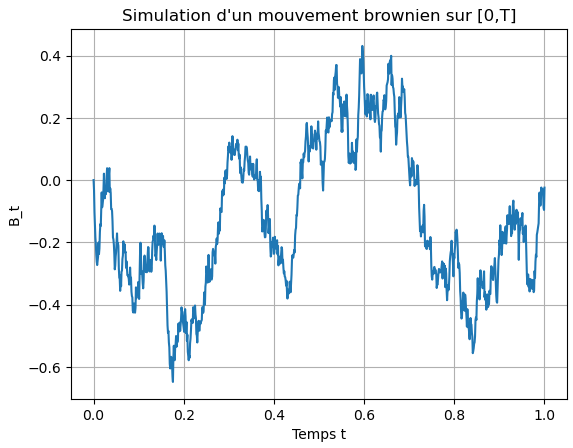
\includegraphics[width=0.75\textwidth]{figure_brownien.png}
    \caption{Simulation d’un mouvement brownien sur l’intervalle $[0,T]$.}
    \label{fig:brownien}
\end{figure}

On observe que la trajectoire fluctue de manière irrégulière autour de zéro. Cette trajectoire servira ensuite à construire les trajectoires approchées de l’EDS.

\subsection{Simulation d’une EDS simple}

Nous considérons d’abord une EDS simple de la forme
\[
dX_t = \mu\,dt + \sigma\,dB_t,
\]
où $\mu$ et $\sigma$ sont des constantes.

Dans ce cas, le coefficient de dérive est donné par
\[
b(x)=\mu,
\]
et le coefficient de diffusion est donné par
\[
\sigma(x)=\sigma.
\]

Le schéma d’Euler-Maruyama devient alors
\[
X_{k+1}=X_k+\mu h+\sigma \Delta B_k.
\]

\begin{figure}[H]
    \centering
    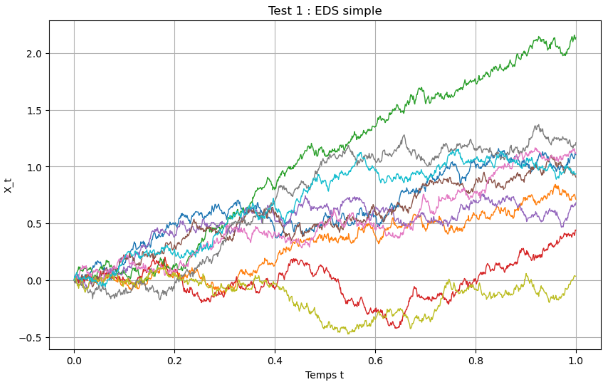
\includegraphics[width=0.75\textwidth]{figure_eds_simple.png}
    \caption{Simulation de plusieurs trajectoires d’une EDS simple.}
    \label{fig:eds_simple}
\end{figure}

Lorsque $\mu>0$, les trajectoires ont globalement tendance à augmenter. Cependant, elles restent perturbées par le terme aléatoire $\sigma dB_t$. On remarque également que plus le coefficient de diffusion est grand, plus les trajectoires sont dispersées.

\subsection{Cas d’un coefficient de diffusion non lipschitzien : $\sigma(x)=\sqrt{x}$}

Nous étudions ensuite le cas
\[
\sigma(x)=\sqrt{x}.
\]

Ce cas est intéressant car la fonction $x\mapsto \sqrt{x}$ n’est pas lipschitzienne en zéro. De plus, elle n’est définie que pour $x\geq 0$. Or, dans une simulation numérique, le schéma d’Euler-Maruyama explicite peut produire temporairement des valeurs négatives, même si la solution théorique est censée rester positive.

En effet, le schéma explicite classique s’écrit
\[
X_{k+1}
=
X_k
+
b(X_k)h
+
\sqrt{X_k}\Delta B_k.
\]

À cause du terme aléatoire $\Delta B_k$, il est possible que la valeur approchée $X_{k+1}$ devienne négative. Dans ce cas, le calcul de la racine carrée au pas suivant n’est plus possible.

Une première correction consisterait à remplacer les valeurs négatives par zéro. Cependant, cette méthode peut provoquer un effet artificiel d’écrasement en zéro : certaines trajectoires peuvent rester bloquées près de zéro à cause du schéma numérique.

Pour éviter ce problème, nous utilisons une variante positive du schéma. L’idée est de traiter le terme en racine de manière semi-implicite :
\[
X_{k+1}
=
X_k
+
b(X_k)h
+
\sqrt{X_{k+1}}\Delta B_k.
\]

On pose alors
\[
Y_{k+1}=\sqrt{X_{k+1}}.
\]

Comme $X_{k+1}=Y_{k+1}^2$, on obtient
\[
Y_{k+1}^2
-
\Delta B_kY_{k+1}
-
\bigl(X_k+b(X_k)h\bigr)
=
0.
\]

On conserve la racine positive :
\[
Y_{k+1}
=
\frac{\Delta B_k+\sqrt{(\Delta B_k)^2+4\bigl(X_k+b(X_k)h\bigr)}}{2}.
\]

On définit ensuite
\[
X_{k+1}=Y_{k+1}^2.
\]

Ce schéma construit donc directement une valeur positive pour $X_{k+1}$, sans projeter brutalement la trajectoire sur zéro.

\begin{figure}[H]
    \centering
    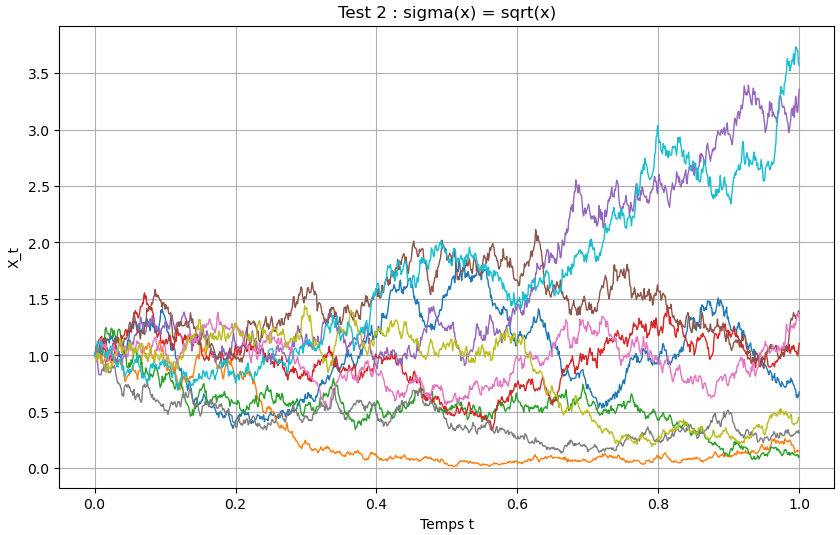
\includegraphics[width=0.75\textwidth]{figure_sigma_racine.png}
    \caption{Simulation avec $\sigma(x)=\sqrt{x}$ en utilisant un schéma positif semi-implicite.}
    \label{fig:sigma_racine}
\end{figure}

Cette correction permet d’éviter les erreurs numériques liées au calcul de la racine carrée d’un nombre négatif. Les trajectoires restent positives ou nulles et peuvent s’approcher de zéro selon les réalisations du mouvement brownien, sans être artificiellement bloquées en zéro.

\subsection{Modèle CIR réfléchi en zéro}

Nous avons également simulé un modèle de type CIR simplifié :
\[
dX_t = \sigma\sqrt{X_t}\,dB_t + \delta\,dt.
\]

Dans ce modèle, le coefficient de diffusion dépend de $\sqrt{X_t}$. Comme précédemment, le schéma numérique peut produire des valeurs négatives. Pour éviter que le coefficient de diffusion ne soit pas défini, nous utilisons une version réfléchie en zéro.

Concrètement, on remplace
\[
\sqrt{X_k}
\]
par
\[
\sqrt{|X_k|}.
\]

Le schéma numérique utilisé est donc de la forme
\[
X_{k+1}
=
X_k
+
\delta h
+
\sigma\sqrt{|X_k|}\Delta B_k.
\]

\begin{figure}[H]
    \centering
    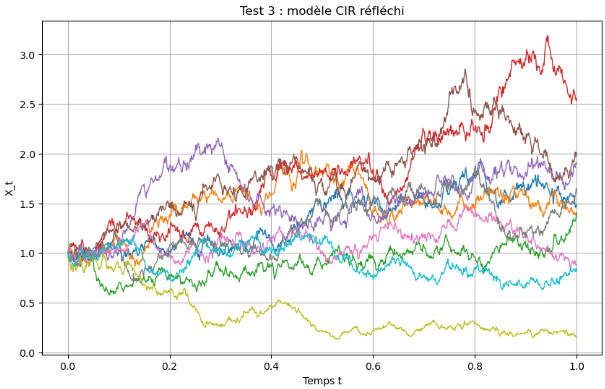
\includegraphics[width=0.75\textwidth]{figure_cir_reflechi.png}
    \caption{Simulation du modèle CIR réfléchi en zéro.}
    \label{fig:cir_reflechi}
\end{figure}

Cette méthode permet de poursuivre la simulation même lorsque le schéma produit une valeur négative. La réflexion en zéro est donc une correction numérique qui permet d’obtenir des trajectoires exploitables.

\subsection{Convergence de l’EDS vers l’EDO lorsque le coefficient de diffusion tend vers zéro}

Nous avons ensuite étudié la convergence d’une EDS vers une EDO lorsque le coefficient de diffusion tend uniformément vers zéro.

On considère une famille d’EDS indexée par un paramètre $\varepsilon>0$ :
\[
dX_t^\varepsilon
=
b(X_t^\varepsilon)\,dt
+
\varepsilon\sigma(X_t^\varepsilon)\,dB_t.
\]

Lorsque $\varepsilon$ tend vers zéro, le coefficient de diffusion
\[
\sigma_\varepsilon(x)=\varepsilon\sigma(x)
\]
tend uniformément vers zéro, à condition que $\sigma$ soit bornée.

L’EDS se rapproche alors de l’EDO déterministe :
\[
dx_t=b(x_t)\,dt.
\]

Pour quantifier cette convergence, nous avons calculé l’erreur uniforme
\[
\sup_{0\leq t\leq T}|X_t^\varepsilon-x_t|,
\]
où $(x_t)_{t\in[0,T]}$ désigne la solution de l’EDO.

Une borne discrète simplifiée utilisée dans les simulations est de la forme
\[
\sup_{0\leq t\leq T}|X_t^\varepsilon-x_t|
\leq
e^{LT}\|\sigma_\varepsilon\|_\infty
\sum_{k=0}^{M-1}|\Delta B_k|,
\]
où $L$ est une constante de Lipschitz associée à $b$.

Comme
\[
\sigma_\varepsilon(x)=\varepsilon\sigma(x),
\]
et si
\[
\|\sigma\|_\infty\leq C,
\]
alors
\[
\|\sigma_\varepsilon\|_\infty\leq \varepsilon C.
\]

On obtient donc une borne de l’ordre de $\varepsilon$ :
\[
\sup_{0\leq t\leq T}|X_t^\varepsilon-x_t|
\leq
e^{LT}\varepsilon C
\sum_{k=0}^{M-1}|\Delta B_k|.
\]

Dans un premier temps, nous avons représenté les trajectoires simulées pour différentes valeurs de $\varepsilon$, ainsi que la solution de l’EDO associée.

\begin{figure}[H]
    \centering
    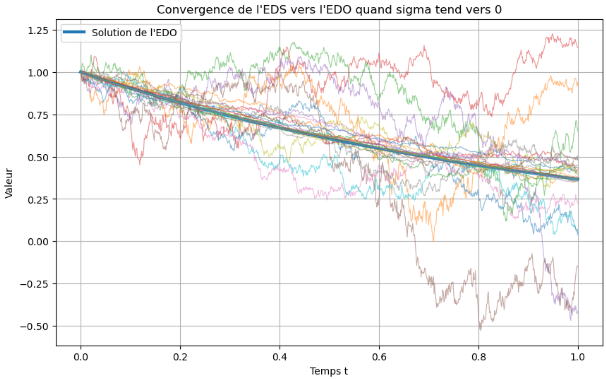
\includegraphics[width=0.75\textwidth]{figure_convergence_edo.png}
    \caption{Convergence des trajectoires de l’EDS vers la solution de l’EDO lorsque $\varepsilon\to 0$.}
    \label{fig:convergence_edo}
\end{figure}

Les résultats numériques montrent que lorsque $\varepsilon$ diminue, les trajectoires de l’EDS se rapprochent de la solution de l’EDO. Cela illustre le fait que la disparition progressive du coefficient de diffusion réduit l’influence du bruit brownien.

Afin de quantifier plus précisément cette convergence, nous avons ensuite calculé, pour chaque valeur de $\varepsilon$, l’erreur moyenne
\[
\mathbb{E}\left[\sup_{0\leq t\leq T}|X_t^\varepsilon-x_t|\right].
\]

En pratique, cette espérance est approchée par une moyenne empirique sur les $N$ trajectoires simulées. Autrement dit, si $X^{\varepsilon,i}$ désigne la $i$-ème trajectoire simulée, l’erreur moyenne est approximée par
\[
\frac{1}{N}\sum_{i=1}^N
\sup_{0\leq t\leq T}
\left|X_t^{\varepsilon,i}-x_t\right|.
\]

Nous avons aussi calculé une borne numérique pour chaque trajectoire simulée. Pour une trajectoire donnée, cette borne est définie par
\[
e^{LT}\varepsilon C
\sum_{k=0}^{M-1}|\Delta B_k^{\,i}|,
\]
où $\Delta B_k^{\,i}$ désigne le $k$-ième accroissement brownien utilisé pour simuler la $i$-ème trajectoire.

La borne moyenne correspond donc à la moyenne empirique de ces bornes sur les $N$ trajectoires simulées :
\[
\frac{1}{N}\sum_{i=1}^N
\left(
e^{LT}\varepsilon C
\sum_{k=0}^{M-1}|\Delta B_k^{\,i}|
\right).
\]

Ainsi, la borne moyenne représente une majoration numérique moyenne de l’erreur uniforme. Elle permet de vérifier que la borne décroît lorsque $\varepsilon$ diminue, comme attendu théoriquement.

\begin{figure}[H]
    \centering
    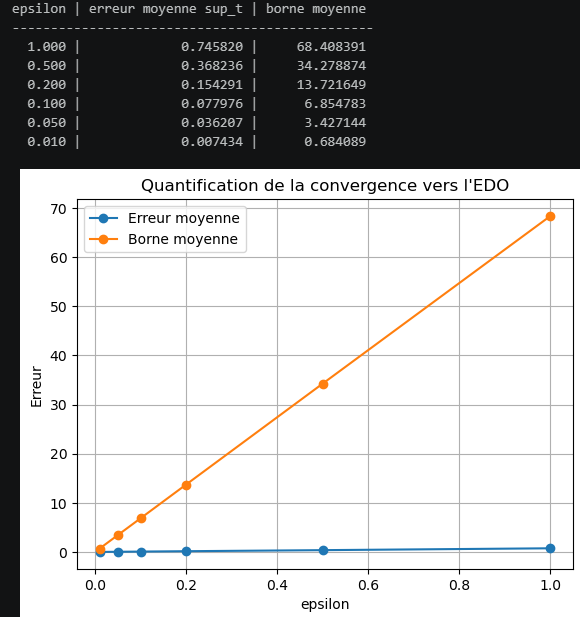
\includegraphics[width=0.75\textwidth]{figure_quantification_convergence.png}
    \caption{Quantification de la convergence vers l’EDO : erreur moyenne et borne moyenne en fonction de $\varepsilon$.}
    \label{fig:quantification_convergence}
\end{figure}

Le graphique montre que l’erreur moyenne diminue lorsque $\varepsilon$ tend vers zéro. Par exemple, pour $\varepsilon=1$, l’erreur moyenne est relativement élevée, tandis qu’elle devient très faible pour $\varepsilon=0.01$. Cela confirme numériquement que la solution de l’EDS converge vers celle de l’EDO lorsque le coefficient de diffusion tend uniformément vers zéro.

On remarque également que la borne moyenne décroît avec $\varepsilon$. Elle est plus grande que l’erreur moyenne observée, ce qui est normal : une borne donne une majoration de l’erreur, mais elle n’est pas nécessairement optimale. L’important est qu’elle diminue elle aussi lorsque $\varepsilon$ diminue, ce qui confirme l’ordre de grandeur attendu.

\subsection{Comparaison des schémas d’Euler-Maruyama et de Milstein}

Enfin, nous avons comparé le schéma d’Euler-Maruyama avec le schéma de Milstein. L’objectif est d’étudier numériquement l’ordre de convergence de ces deux méthodes.

On considère une EDS générale de la forme
\[
dX_t = b(X_t)\,dt + \sigma(X_t)\,dB_t.
\]

Le schéma d’Euler-Maruyama associé est donné par
\[
X_{k+1}
=
X_k
+
b(X_k)h
+
\sigma(X_k)\Delta B_k,
\]
où
\[
\Delta B_k = B_{t_{k+1}}-B_{t_k}
\sim \mathcal{N}(0,h).
\]

Le schéma de Milstein est une amélioration du schéma d’Euler-Maruyama. Il ajoute un terme correctif qui fait intervenir la dérivée du coefficient de diffusion. Lorsque $\sigma$ est dérivable, le schéma de Milstein s’écrit :
\[
X_{k+1}
=
X_k
+
b(X_k)h
+
\sigma(X_k)\Delta B_k
+
\frac{1}{2}\sigma(X_k)\sigma'(X_k)
\left((\Delta B_k)^2-h\right).
\]

Le terme supplémentaire
\[
\frac{1}{2}\sigma(X_k)\sigma'(X_k)
\left((\Delta B_k)^2-h\right)
\]
permet d’améliorer la précision de l’approximation. C’est pourquoi le schéma de Milstein possède en général un meilleur ordre de convergence forte que le schéma d’Euler-Maruyama.

Pour comparer les deux schémas, nous avons choisi une EDS dont la solution exacte est connue : le mouvement brownien géométrique.

On considère l’EDS
\[
dX_t = \mu X_t\,dt + \sigma X_t\,dB_t,
\qquad X_0=x_0.
\]

Dans ce cas, on a
\[
b(x)=\mu x
\]
et
\[
\sigma(x)=\sigma x.
\]

La dérivée du coefficient de diffusion est donc
\[
\sigma'(x)=\sigma.
\]

La solution exacte est donnée par
\[
X_t
=
x_0
\exp\left(
\left(\mu-\frac{\sigma^2}{2}\right)t+\sigma B_t
\right).
\]

Pour cette EDS, le schéma d’Euler-Maruyama devient
\[
X_{k+1}
=
X_k
+
\mu X_k h
+
\sigma X_k \Delta B_k.
\]

En appliquant la formule générale du schéma de Milstein, on obtient
\[
X_{k+1}
=
X_k
+
\mu X_k h
+
\sigma X_k \Delta B_k
+
\frac{1}{2}\sigma^2X_k\left((\Delta B_k)^2-h\right).
\]

La différence entre les deux schémas vient donc du terme correctif
\[
\frac{1}{2}\sigma^2X_k\left((\Delta B_k)^2-h\right).
\]

Pour comparer les deux méthodes, nous calculons l’erreur au temps final :
\[
|X_T-X_T^{\text{approx}}|,
\]
où $X_T$ désigne la solution exacte et $X_T^{\text{approx}}$ la valeur approchée obtenue par Euler-Maruyama ou par Milstein.

Cette erreur est ensuite moyennée sur plusieurs trajectoires simulées. On répète cette expérience pour plusieurs valeurs du pas de temps $h$, puis on trace l’erreur en fonction de $h$ en échelle logarithmique.

\begin{figure}[H]
    \centering
    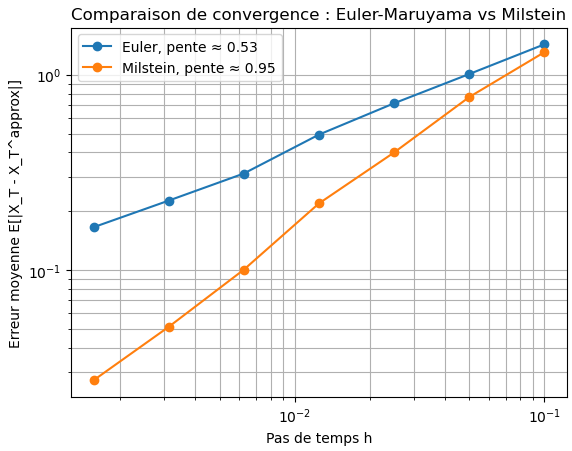
\includegraphics[width=0.75\textwidth]{figure_euler_milstein_loglog.png}
    \caption{Comparaison de la convergence des schémas d’Euler-Maruyama et de Milstein en échelle log-log.}
    \label{fig:euler_milstein}
\end{figure}

Sur un graphique en échelle log-log, si l’erreur se comporte comme
\[
\text{erreur}(h)\simeq Ch^\alpha,
\]
alors on a
\[
\log(\text{erreur}(h))
\simeq
\log(C)+\alpha\log(h).
\]

La pente de la droite obtenue correspond donc à l’ordre de convergence du schéma.

Numériquement, on s’attend à observer une pente proche de $1/2$ pour le schéma d’Euler-Maruyama et une pente proche de $1$ pour le schéma de Milstein. Le graphique confirme que le schéma de Milstein converge plus rapidement que le schéma d’Euler-Maruyama.

\subsection{Conclusion des résultats numériques}

Les simulations numériques montrent que le schéma d’Euler-Maruyama permet d’approximer simplement les trajectoires d’une équation différentielle stochastique. La simulation du mouvement brownien permet d’abord de visualiser le bruit aléatoire intervenant dans l’EDS.

Les exemples étudiés mettent aussi en évidence certaines difficultés numériques. En particulier, lorsque le coefficient de diffusion est donné par $\sigma(x)=\sqrt{x}$, le schéma peut produire des valeurs négatives. Il est alors nécessaire d’utiliser une correction, comme la partie positive ou la réflexion en zéro.

Les simulations montrent également que lorsque le coefficient de diffusion tend uniformément vers zéro, les trajectoires de l’EDS se rapprochent de la solution de l’EDO associée. Enfin, la comparaison entre les schémas d’Euler-Maruyama et de Milstein montre que le schéma de Milstein possède un meilleur ordre de convergence dans le cas du mouvement brownien géométrique.

\section*{Conclusion}

Ce projet a permis de mieux comprendre les équations différentielles stochastiques, aussi bien sur le plan théorique que numérique. La démonstration du théorème d'existence et d'unicité par itération de Picard est assez technique mais elle repose sur des arguments relativement naturels une fois qu'on a bien en tête la structure de l'espace $M^2$. Les résultats de stabilité : convergence vers une EDO et dépendance en la condition initiale, s'obtiennent tous les deux par le même outil, le lemme de Gronwall.

Du côté numérique, le schéma d'Euler-Maruyama est simple à coder mais il faut faire attention à certains cas particuliers. Quand le coefficient de diffusion est par exemple $\sigma(x)=\sqrt{x}$, le schéma peut produire des valeurs négatives et il faut prévoir une correction. La comparaison avec Milstein montre clairement que ce dernier converge plus vite (ordre $1$ contre $1/2$), même si la différence n'est pas toujours énorme en pratique pour des pas de temps raisonnables.

En résumé, les simulations confirment bien les résultats théoriques et permettent de les visualiser concrètement, ce qui aide à mieux les appréhender.

\section*{Bibliographie}

\begin{itemize}
    \item F. Comets et T. Meyre, \textit{Calcul stochastique et modèles de diffusions}, Dunod.

    \item E. Altman, \textit{Cours de calcul stochastique}.
\end{itemize}

\section*{Annexe : code Python et exécutable}

Cette annexe contient le code Python complet utilisé pour les simulations. L’exécutable associé est également fourni avec le rapport.

Nous présentons également une capture de l’interface de l’exécutable, afin de montrer à quoi ressemble l’application une fois lancée.

% Insérer ici la capture de l'interface de l'exécutable
\begin{figure}[H]
    \centering
    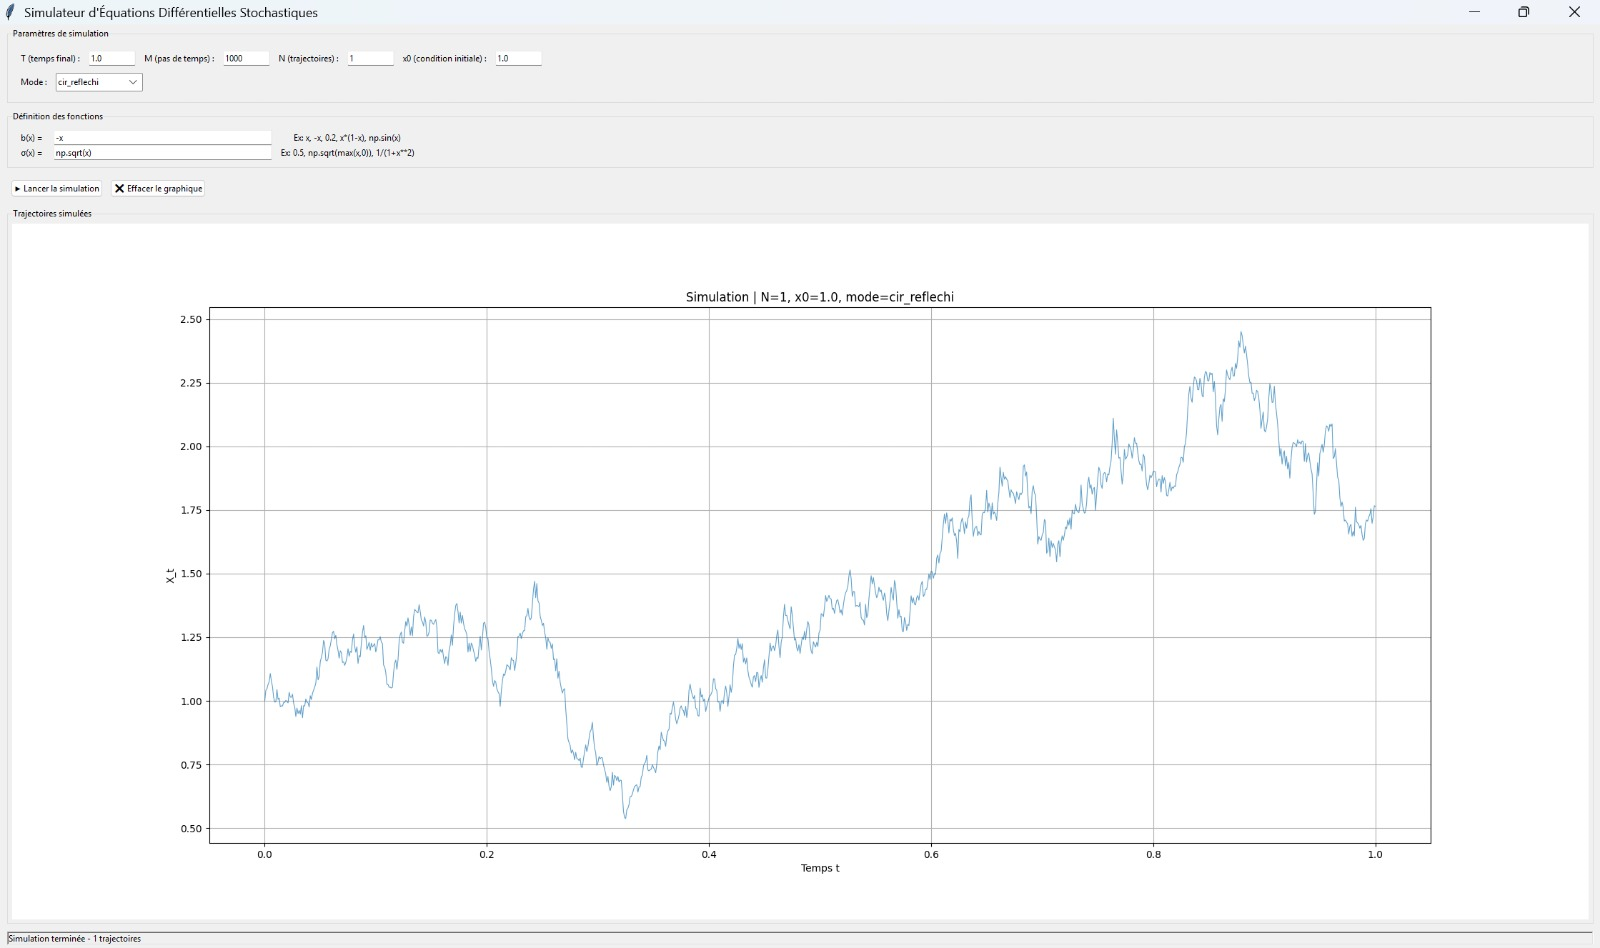
\includegraphics[width=0.75\textwidth]{interface_executable.png}
    \caption{Interface de l’exécutable utilisé pour lancer les simulations numériques.}
    \label{fig:interface_executable}
\end{figure}

\lstinputlisting{code_PNI.py}

\end{document}